% !Mode:: "TeX:UTF-8"
%!TEX program  = xelatex

% \documentclass{cumcmthesis}
\documentclass[withoutpreface,bwprint]{cumcmthesis} %去掉封面与编号页
\usepackage{url}
\usepackage{graphicx}
\usepackage{float}
\usepackage{threeparttable}
\newcommand{\upcite}[1]{\textsuperscript{\textsuperscript{\cite{#1}}}}

\title{“拍照赚钱”的任务定价}
\tihao{A}
\baominghao{4321}
\schoolname{XX大学}
\membera{zstar}
\memberb{向左}
\memberc{哈哈}
\supervisor{老师}
\yearinput{2021}
\monthinput{08}
\dayinput{22}

\begin{document}

 \maketitle
 \begin{abstract}

随着劳务众包平台的兴起,如何对任务进行合理定价成为平台的重要工作。本文依据题目所给数据研究现有定价规律,并建立模型进行优化。

对于问题一,首先我们通过数据预处理将\textbf{13}个异常会员值进行剔除。之后,运用\textbf{墨卡托投影法},将所有数据的经纬度转换成平面坐标。然后,我们用\textbf{k-means}聚类方法对任务点作了聚类分析,计算了偏僻程度,会员密度,任务密度和任务标价的\textbf{Pearson相关系数},并构建\textbf{多元线性回归模型}来拟合任务标价规律。最后,我们分析了任务未完成的3个原因。

对于问题二,我们结合当地的经济发展情况和任务、会员之间的距离,定义了任务对会员\textbf{吸引力}这个概念。之后,我们建立\textbf{多目标规划模型},求解出了新的任务标价和任务完成情况。新方案比原方案成本降低\textbf{13.07\%},完成率提升\textbf{29.71\%}。

对于问题三,我们首先求出任务之间的距离矩阵,然后通过\textbf{层次聚类法}对相邻任务进行打包。之后,对第二问的多目标优化模型参数进行修正,求得新的方案。新方案比问题二的方案成本降低\textbf{8.7\%},完成率提升\textbf{6.13\%}。

对于第四问,我们先用层次聚类法对任务进行打包。之后,通过\textbf{BP神经网络}模型,以经纬度作为输入量,任务标价、完成情况作为输出量,求得任务定价方案,完成率为\textbf{85.97\%}

最后,我们对模型进行了优缺点分析和推广。


\keywords{墨卡托投影法\quad  层次聚类法\quad   多元线性回归模型\quad  多目标优化模型}
\end{abstract}

%目录(可要可不要)
\tableofcontents


\section{问题重述}

\subsection{背景资料}

近年来,随着互联网技术的高速发展,网络已经融入了我们生活的方方面面。
“拍照赚钱”是移动互联网下的一种自助式服务模式,有多家公司依托移动互联网
建立了服务平台,如“拍拍赚”、“蚂蚁威客”、“美团拍客”等等。用户下载 APP,注册
成为 APP 的会员,然后从 APP 上领取需要拍照的任务(比如上超市去检查某种商品的
上架情况),赚取 APP 对任务所标定的酬金。这种基于移动互联网的自助式劳务众包平
台,为企业提供各种商业检查和信息搜集,相比传统的市场调查方式可以大大节省调查
成本,而且有效地保证了调查数据真实性,缩短了调查的周期。因此 APP 成为该平台运
行的核心,而 APP 中的任务定价又是其核心要素。如果定价不合理,有的任务就会无人
问津,而导致商品检查的失败。

\subsection{需要解决的问题}

我们通过分析相关数据,运用数学思想,建立数学模型来研究拍照软件定价中的下
列问题:

(1) 研究附件一中项目的任务定价规律,分析任务未完成的原因。

(2) 为附件一中的项目设计新的任务定价方案,并和原方案进行比较。

(3) 实际情况下,多个任务可能因为位置比较集中,导致用户会争相选择,一种考虑是将这些任务联合在一起打包发布。在这种考虑下,如何修改前面的定价模型,对最终的任务完成情况又有什么影响?

(4) 对附件三中的新项目给出你的任务定价方案,并评价该方案的实施效果。

\section{问题分析}

\subsection{问题一分析}

问题一要求研究附件一中项目的任务定价规律,分析任务未完成的原因。我们的思路图如下所示:

\begin{figure}[H]
	\centering
	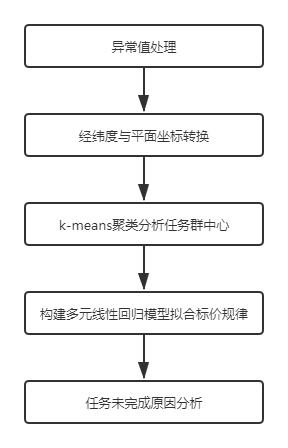
\includegraphics[width=8cm]{../../img/12.png}
	\caption{问题一流程图}
\end{figure}

\subsection{问题二分析}
题目要求为附件一中的项目设计新的任务定价方案,并和原方案进行比较。我们结合当地的经济发展情况和任务、会员之间的距离,定义了任务对会员吸引力这个概念。之后,我们建立多目标规划模型,求解新的任务标价和任务完成情况。

\subsection{问题三分析}
题目要求建立打包模式下的任务标价模型。我们首先求出任务之间的距离矩阵,然后通过层次聚类法对相邻任务进行打包。之后,对第二问的多目标优化模型参数进行修正,求得新的方案。

\subsection{问题四分析}
题目要求对附件三中的新项目给出你的任务定价方案,并评价该方案的实施效果。我们先用层次聚类法对任务进行打包。之后,通过BP神经网络模型,以经纬度作为输入量,任务标价、完成情况作为输出量,求得任务定价方案。

\section{模型的假设}

\begin{itemize}
\item 假设所给任务难易程度均相同且都可实现。
\item 忽略天气、交通状况等不确定因素对任务定价的影响。
\item 认为附件中所有数据均真实可靠。
\end{itemize}

\section{符号说明}
\begin{center}
\begin{tabular}{cc}
 \hline
 \makebox[0.3\textwidth][c]{符号}	&  \makebox[0.4\textwidth][c]{意义} \\ \hline
$L_n$	    & 经度\\ \hline
$L_a$	    & 纬度 \\ \hline
$d_i$	    & 任务i的偏僻程度 \\ \hline
$\rho_j$	    & 会员密度  \\ \hline
$\rho_i$	    & 任务密度  \\ \hline
$L_a$	    & 纬度 \\ \hline
$a_{ij}$	    & 任务i对会员j的吸引力 \\ \hline
$a_i$	    & 吸引力阈值 \\ \hline
$p_i$	    & 任务i的标价 \\ \hline
\end{tabular}
\end{center}



\section{模型的建立与求解}
\subsection{问题一模型的建立及求解}
\subsubsection{模型的准备:数据可视化与处理}
根据附件一和附件二的数据,我们可以将经纬度投射到地图上,以便更为直观地探究任务以及会员分部的特点。

\textbf{1.任务点分布可视化}

我们将附件一的任务数据在地图上标记出来,如下图所示:

\begin{figure}[H]
	\small
	\centering
	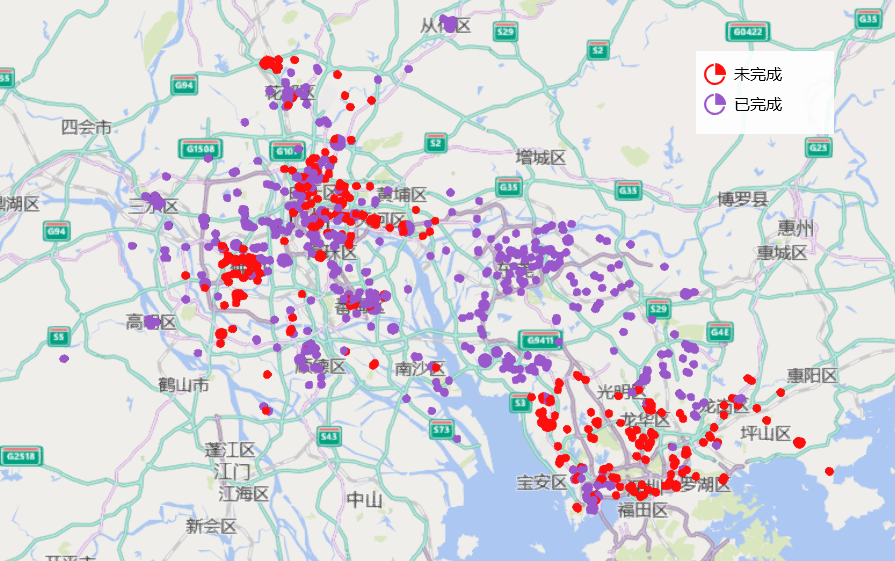
\includegraphics[width=12cm]{../../img/1.png}
	\caption{任务分布图} 
\end{figure}

从图中可以发现,任务的分布主要集中在广东省的广州、深圳、佛山、东莞四个城市,并且东莞地区的任务完成率最高,深圳地区的任务完成率最低。

\textbf{2.会员分布可视化}

我们将附件二的会员数据在地图上标记出来,如下图所示:

\begin{figure}[H]
	\small
	\centering
	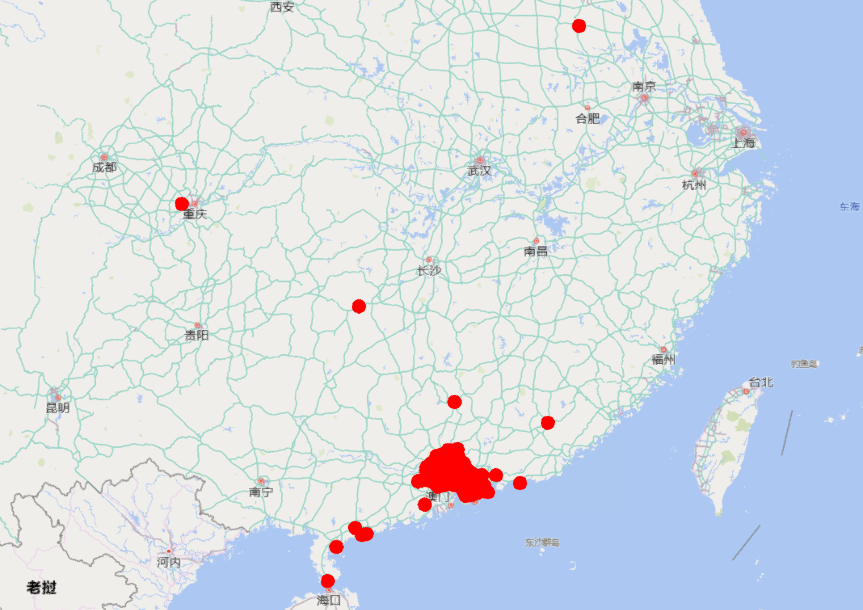
\includegraphics[width=12cm]{../../img/2.png}
	\caption{剔除异常数据前的会员分布图} 
\end{figure}

从图中可以发现,13个会员的位置数据异常,远离广东省,因此将其进行剔除。这13个会员的编号分别为B00005、B00006、B00007、B00022、B00033、B00039、B00048、B00081、B00136、B00472、B001708、B01727、B01796。

剔除之后,我们可以再将会员的位置数据可视化,如下图所示:
\begin{figure}[H]
	\small
	\centering
	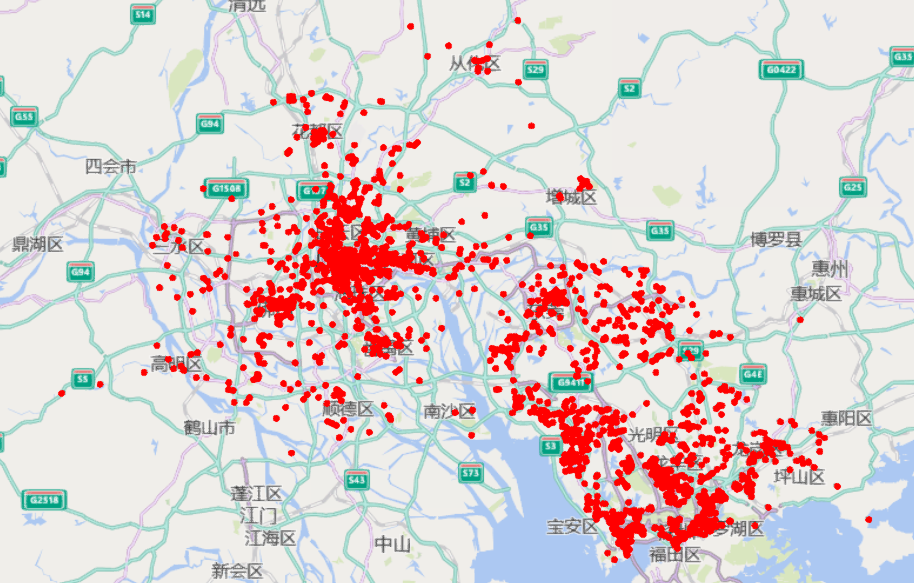
\includegraphics[width=12cm]{../../img/3.png}
	\caption{剔除异常数据后的会员分布图} 
\end{figure}

从图中我们可以看出,会员的分布情况和任务的分布情况大致相当,因此我们可以推测,任务的标价和完成率和会员的分布情况存在一定关系。


\textbf{3.经纬度与平面坐标转换}

由于题目中给的均是经纬度数据,而通过经纬度计算两点之间的距离相对麻烦。因此,我们首先通过墨卡托投影法将所有点的经纬度数据转换成平面上的二维坐标。

投影公式如下:

\begin{equation}
x = \frac{{{L_n} \times \pi }}{{180}} \times {R_E}
\end{equation}

\begin{equation}
y = \frac{{{R_E}}}{2} \times \log (\frac{{1 + \sin (a)}}{{1 - \sin (a)}})
\end{equation}

式中,${L_n}$为经度,${L_a}$为纬度,${R_E}$表示地球半径,取${R_E}$=6378.137,a表示弧度,${a = \frac{{{L_a} \times \pi }}{{180}}}$。

为了进一步简化计算,我们取所有坐标点的均值点作为坐标原点(0,0)。

\textbf{4.任务点的聚类分析}

在上面的可视化分析中,我们发现所有任务点主要集中在4个大城市周围。因此,我们使用K-means算法对任务坐标点进行聚类分析,分成4簇,画出的聚类图如下所示:

\begin{figure}[H]
	\small
	\centering
	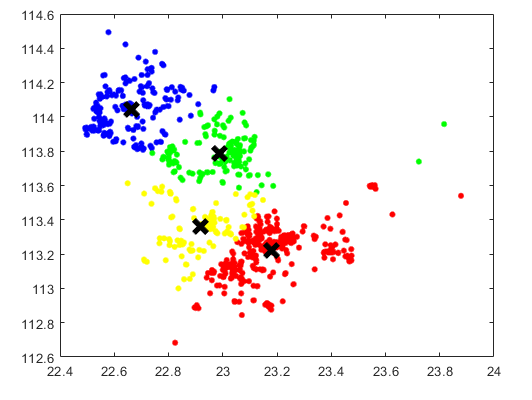
\includegraphics[width=12cm]{../../img/4.png}
	\caption{任务分布聚类图} 
\end{figure}

得到四个聚类中心的经纬度坐标为:


\begin{table}[H]
	\centering
	\caption{聚类中心的经纬度坐标}
	\begin{tabular}{|c|c|c|c|c|}
		\hline
		聚类中心 & 1         & 2         & 3         & 4         \\ \hline
		经度   & 23.18137  & 22.66239  & 22.98919  & 22.98919  \\ \hline
		纬度   & 113.21833 & 114.04244 & 113.78511 & 113.36159 \\ \hline
	\end{tabular}
\end{table}


我们发现这四个聚类中心的位置和可视化分析中4个大城市的位置接近,这和我们的直观判断相一致。

\subsubsection{任务标价的影响因素}
\textbf{1.偏僻程度${d_i}$}

我们认为,当一个任务距离市中心越近时,会员完成该任务就会越方便,该任务就更容易被完成,因此,该任务的标价应当适当降低。而当一个任务距离市中心越远时,交通就越不方便,会员完成该任务就越困难,相应的,该任务的标价应当适当提高,以此来激励更多人前来完成。于是我们定义一个偏僻程度这个变量,来刻画任务距离聚类中心的远近程度。偏僻程度越大,该任务距聚类中心越远,也就越偏僻。

\begin{equation}
{d_i} = \sqrt {{{({x_i} - {x_o})}^2} + {{({y_i} - {y_o})}^2}} 
\end{equation}

式中,$({x_i} ,{y_i})$表示当前任务坐标,$({x_o} ,{y_o})$表示当前距离任务点最近的聚类中心的坐标。

\textbf{2.会员密度${\rho_j}$}

我们认为,当一个任务周边会员较多时,该任务更容易被会员预定并且完成,该任务的标价应当适当降低。而当一个任务周边会员较少时,该任务被预定的几率降低,该任务的标价应当适当提高,以此来激励会员前来完成。因此,我们定义会员密度这个变量,来刻画任务周边会员的聚集程度。

\begin{equation}
{\rho _j} = \frac{{{n_k}}}{{\sum\limits_{j = 1}^n {{n_j}} }}
\end{equation}

式中,分母为会员总数,${n_k}$为任务点5km之内的会员数。

\textbf{3.任务密度${\rho_i}$}

我们认为,当一个任务周边有多个任务时,会员更容易会来预定该任务,以便同时可以完成多个邻近的任务,此时该任务的标价应当适当降低。而当一个任务周边的任务数较少时,会员将更不倾向预定该任务,此时该任务的标价应当适当提高。因此,我们定义任务密度这个变量,来刻画任务周边其它任务的密集程度。

\begin{equation}
{\rho _i} = \frac{{{n_p}}}{{\sum\limits_{i = 1}^n {{n_i}} }}
\end{equation}

式中,分母为任务总数,${n_p}$为任务点5km之内的任务数。


\subsubsection{影响因素的相关性分析}

为了探究这三个影响因素对任务标价的影响程度,我们以Pearson相关系数来进行量化分析,Pearson相关系数可以刻画变量与变量之间的线性相关程度。

\begin{equation}
{y=\frac{\mbox{C}ov\left( X,Y \right)}{\sqrt{D\left( X \right)}\; \sqrt{D\left( Y \right)}}}
\end{equation}

计算结果如下表所示:

\begin{table}[H]
	\centering
	\caption{影响因素与任务标价之间的相关系数}
	\begin{tabular}{|c|c|c|c|}
	\hline
	影响因素 & 偏僻程度  & 会员密度   & 任务密度   \\ \hline
	相关系数 & 0.559 & -0.449 & -0.427 \\ \hline
	显著性  & 0.000 & 0.000  & 0.000  \\ \hline
	\end{tabular}
\end{table}
\vspace{-0.8cm}

从表中我们可以得知,三个影响因素与任务标价的线性相关性显著。并且,偏僻程度和任务标价正相关,会员密度与任务密度和任务标价负相关。这说明,任务距离聚类中心越远,任务越偏僻,任务标价越高;任务周边会员密度越大,任务密度越大,周边的会员和任务越多,任务标价越低。这和我们的常识相一致。

\subsubsection{多元线性回归模型}
我们已经分析得知,三个影响因素和任务标价线性相关。因此,我们以偏僻程度${d_i}$、会员密度${\rho_j}$、任务密度${\rho_i}$为自变量,任务标价${p_i}$为因变量,构建多元线性回归模型。

\begin{equation}
{p_i} = {\alpha _1}{d_i} + {\alpha _2}{\rho _j} + {\alpha _3}{\rho _i} + \beta 
\end{equation}

我们通过SPSS软件进行求解,结果如下:

\begin{equation}
{p_i} = 5.291{d_i} - 4.900{\rho _j} - 2.536{\rho _i} + 70.459
\end{equation}


F检验值为80.549,p值为0.000<0.05,说明支持原假设,线性回归方程显著。

\subsubsection{任务未完成的原因}

我们筛选出未完成的任务数,将相关数据代入上面的任务定价模型,求得计算定价,并与实际定价作对比,对比结果如下图所示:

\begin{figure}[H]
	\small
	\centering
	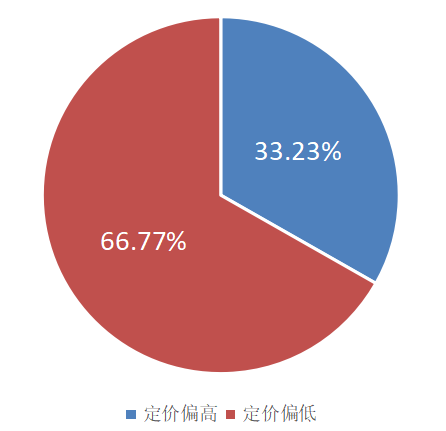
\includegraphics[width=8cm]{../../img/5.png}
	\caption{未完成的任务定价评估} 
\end{figure}

从图中我们可以发现,大部分的任务定价都偏低。因此,我们推测任务定价偏低是任务未完成的主要原因。

此外,我们发现东莞地区任务完成率较高,深圳地区任务完成率较低。所以,任务未完成的原因可能还与当地的经济发展状况相关;同时,交通、环境等情况也会对会员完成任务造成影响。

因此,我们将任务未完成的原因进行归纳,可总结为以下三点:

1.任务未完成的主要原因是定价偏低,会员积极性不足。

2.当地经济条件影响会员对任务标价的预估,使任务完成情况具有区域性。

3.受到其它不确定因素的影响,比如,天气、环境、交通、会员个人因素等。


\subsection{问题二模型的建立及求解}
\subsubsection{模型的准备}
问题一的定价模型主要以任务为中心来进行标价的确定,我们打算以会员为中心来对标价模型进行改进。

\textbf{1.经济需求度${e_i}$}

在可视化分析中,我们发现不同地区的任务完成率不太一样。经济较为发达的广州深圳地区,人们对任务佣金需求度低,导致任务完成率低,而在经济相对落后的东莞地区,人们对任务佣金需求度高,导致任务完成率高。

通过查阅相关资料,我们查到了广州、深圳、佛山、东莞2020年人均GDP信息,如下表所示:

\begin{table}[H]
	\centering
	\caption{四个城市的人均GDP信息}
	\begin{tabular}{|c|c|c|c|c|}
	\hline
	城市       & 广东    & 深圳     & 佛山     & 东莞     \\ \hline
	人均GDP(元) & 94172 & 203489 & 133850 & 112507 \\ \hline
	\end{tabular}
\end{table}


为了刻画会员对经济的需求程度,我们定义经济需求度为当地人均GDP的倒数:

\begin{equation}
{e_i} = \frac{1}{{{G_i}}}
\end{equation}

式中,${G_i}$代表第i个城市的人均GDP。

\textbf{2.吸引力${a_{ij}}$}

从用户的角度考虑,我们定义吸引力来衡量会员预定任务的积极性。任务对用户的吸引力越大,用户完成任务的积极性越高。我们参考万有引力的公式,对吸引力作如下定义:

\begin{equation}
{a_{ij}} = \frac{{K{e_j}{p_i}}}{{{r_{ij}}^2}}
\end{equation}

式中,${a_{ij}}$表示任务i对会员j的吸引力,${p_i}$表示任务标价,${r_{ij}}$表示任务i距离会员j的距离,K为修正参数,通过修正参数,可以将吸引力的取值范围限定在[0,1]之间。当吸引力的值接近于0时,说明该任务对会员毫无吸引力;当吸引力的值接近于1时,说明这个任务非常具有吸引力。
	
\textbf{3.吸引力阈值${a_{i}}$}

为了标记任务是否能被完成,我们需要定义吸引力阈值${a_{i}}$:

\begin{equation}
{C_i} = \left\{ \begin{array}{l}
{\rm{1,}}{a_{ij}} \ge {a_i}\\
0,{a_{ij}} < {a_i}
\end{array} \right.
\end{equation}

式中,${C_i}$表示任务是否被完成,当吸引力等于或大于阈值时,会员会选择该任务并完成,当吸引力小于阈值时,该任务将无会员预定,不能被完成。

我们假定阈值${a_i}$为0.5。

%\subsubsection{多目标规划模型}
有了上面的一些定义之后,我们可以建立多目标规划模型。

\textbf{1.目标函数的确定}

对于企业来说,最好的效果是用最少的成本换取最大的收益。
因此我们确定两个目标:最小化成本和最大化完成率。

\begin{equation}
\left\{ \begin{array}{l}
\min \sum\limits_{i = 1}^{835} {{p_i}} \\
\max \sum\limits_{i = 1}^{1864} {{C_i}} 
\end{array} \right.
\end{equation}

\textbf{2.约束条件的确定}

$\bullet$任务标价的范围

附件一中,任务的标价范围为[65,85],为了让任务标价具备一个灵活调节的区间并且防止标价过于夸张,因此需要我们给任务标价限定在[50,100]这个范围之内,即

\begin{equation}
{\rm{50}} \le {\rm{p}}{}_{\rm{i}} \le 100,i = 1,2,...,835
\end{equation}

$\bullet$用户接单的数量

附件二中有每个会员的预订任务限额数据,而任务是根据预订限额所占比例进行配发。因此,每个会员所能接收的任务数上限${{\rm{w}}_{{\rm{imax}}}}$为

\begin{equation}
{{\rm{w}}_{{\rm{imax}}}} = {n_s} \times {m_i},i = 1,2,...,835
\end{equation}

\begin{equation}
{n_s} = n - {n_d}
\end{equation}

式中,${n_d}$表示已经领取的任务数量,n表示任务总数,${n_s}$表示剩余任务数量,${m_i}$表示用户预订限额所占比例。

$\bullet$用户预定任务规则

由于用户开始预定的任务时间不一致,因此我们假定用户预定任务之后,该任务就可被用户完成。时间早的用户先进行任务的预定,任务一旦预定后,就从任务池中移除,不能再被其它用户重复预定。

\begin{equation}
{{\rm{s}}_i} \in {n_s},i = 1,2,...,835
\end{equation}

式中,${s_i}$表示当前用户的预定任务,${n_s}$表示剩余任务数量。

$\bullet$用户预定任务倾向

用户预定任务时,将根据任务对其的吸引力进行排序,选取超过吸引力阈值的任务。

\begin{equation}
{{\rm{s}}_i} = \left\{ \begin{array}{l}
\max ({a_{ij}}),{a_{ij}} > {a_i}\\
i = 1,2,...,835,j = 1,2,...,1864
\end{array} \right.
\end{equation}

$\bullet$冲突任务优先分配

若同一个任务在相同时间被多个用户选取,则该任务将由这些用户中信誉值最高的用户获得。

\begin{equation}
{s_i} = \max ({b_{s1}},{b_{s2}},...,{b_{sn}})
\end{equation}

${s_i}$表示任务的归属,${b_{sn}}$表示同时选取该任务的n个用户的信誉值。

综上,得到定价设计问题的多目标优化模型:

目标函数:
\begin{equation}
\left\{ \begin{array}{l}
\min \sum\limits_{i = 1}^{835} {{p_i}} \\
\max \sum\limits_{i = 1}^{1864} {{C_i}} 
\end{array} \right.
\end{equation}

\begin{equation}
s.t.\left\{ \begin{array}{l}
{\rm{50}} \le {\rm{p}}{}_{\rm{i}} \le 100\\
{a_{ij}} = \frac{{G{n_j}{p_i}}}{{{r_{ij}}^2}}\\
{C_i} = \left\{ \begin{array}{l}
{\rm{1,}}{a_{ij}} \ge {a_i}\\
0,{a_{ij}} < {a_i}
\end{array} \right.\\
{{\rm{w}}_{{\rm{imax}}}} = {n_s} \times {m_i}\\
{n_s} = n - {n_d}\\
{{\rm{s}}_i} \in {n_s}\\
{{\rm{s}}_i} = \max ({a_{ij}}),{a_{ij}} > {a_i}\\
{s_i} = \max ({b_{s1}},{b_{s2}},...,{b_{sn}})
\end{array} \right.,i = 1,2,...,835,j = 1,2,...,1864
\end{equation}

\textbf{3.模型的求解}

由于该模型约束条件较为复杂,直接求解难度较大。因此,我们建立模拟会员抢单的方式,通过蒙特卡洛法进行求解。

具体过程:

1.在任务标价的范围内,随机初始化各个任务标价。

2.计算在该任务标价下每个任务对各个会员的吸引力。

3.对每个会员的预订任务开始时间从早到晚进行排序,若时间相同,则根据每个会员的信誉值从高到低进行排序。

4.计算每个会员的预订任务限额所占比例。

5.根据会员的排序顺序,按会员从高到低的优先级进行任务选取,任务选取的数量上限由预订任务限额所占比例决定。

6.计算该种情况下,所有任务的所需成本和任务的完成率。

7.循环多次,从所有结果中选取最优结果。

\begin{figure}[H]
	\small
	\centering
	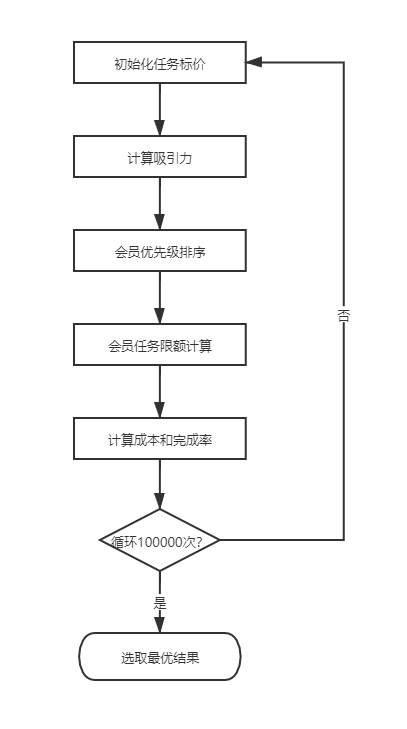
\includegraphics[width=8cm]{../../img/6.png}
	\caption{求解算法过程} 
\end{figure}

通过10万次的模拟,我们得到了最优结果如下表所示:

\begin{table}[H]
	\centering
	\caption{问题二任务标价与执行情况}
	\begin{threeparttable}       
	\begin{tabular}{|c|c|c|c|c|}
	\hline
	任务号码  & 原任务标价 & 原任务执行情况 & 现任务标价 & 现任务执行情况 \\ \hline
	A0001 & 66    & 0       & 51    & 1       \\ \hline
	A0002 & 60    & 0       & 61    & 1       \\ \hline
	A0003 & 60    & 1       & 61    & 1       \\ \hline
	A0004 & 75    & 0       & 59    & 1       \\ \hline
	A0005 & 60    & 0       & 61    & 1       \\ \hline
	\multicolumn{5}{|c|}{......}              \\ \hline
	A0831 & 60    & 0       & 61    & 0       \\ \hline
	A0832 & 72    & 1       & 51    & 1       \\ \hline
	A0833 & 85    & 1       & 66.5  & 1       \\ \hline
	A0834 & 60    & 1       & 61    & 1       \\ \hline
	A0835 & 85    & 1       & 66.5  & 1       \\ \hline
	\end{tabular}
	\begin{tablenotes}
		\footnotesize
		\item 注:由于篇幅有限,这里仅展示部分数据。
	\end{tablenotes}
\end{threeparttable}     
\end{table}


通过计算,新方案成本为49447元,原方案成本为56882.5元,新方案任务完成率为81.08\%,原方案任务完成率为62.51\%。与原方案相比,新方案在成本降低13.07\%的情况下,任务完成率提升29.71\%。由此可见,新方案具有较大改进。


\subsection{问题三模型的建立及求解}
\subsubsection{任务的打包}

\textbf{1.建立任务之间的距离矩阵}

在第一问,我们已经将各个任务点的经纬度坐标转换成了平面的距离坐标。现在我们通过两点之间的欧式距离来获得各任务点的距离矩阵。

\begin{equation}
{d_{ij}} = \sqrt {{{\left( {{x_i} - {x_j}} \right)}^2} + {{\left( {{y_i} - {y_j}} \right)}^2}}
\end{equation}

\begin{equation}
D = \left[ {\begin{array}{*{20}{c}}
	{\rm{0}}&{{d_{12}}}&{...}&{{d_{1835}}}\\
	{{d_{21}}}&{\rm{0}}&{...}&{...}\\
	{...}&{...}&{\rm{0}}&{...}\\
	{{d_{8351}}}&{...}&{...}&{\rm{0}}
	\end{array}} \right]
\end{equation}

\textbf{2.层次聚类法进行任务打包}

为了更好地将任务打包处理,我们采用层次聚类方法。

层次聚类的算法流程:

Step1:将每个任务看作一类,计算两两之间的最小距离。

Step2:将距离最小的两个类合并成一个新类。

Step3:重新计算新类与所有类之间的均值距离。

Step4:重复二三步,直到所有类最后合并为一类。

Step5:结束。

层次聚类法的结果如下图所示:

\begin{figure}[H]
	\small
	\centering
	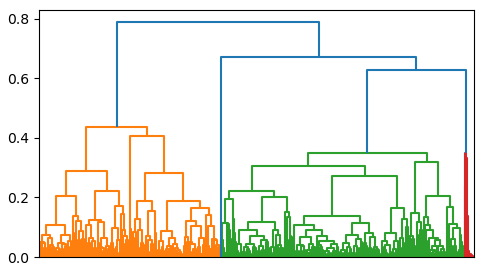
\includegraphics[width=12cm]{../../img/7.png}
	\caption{整体层次聚类法结果} 
\end{figure}

考虑到如果将过多的任务打包,让一个用户来预定,那可能会造成任务无法被全部完成,并且也对其他用户来说,也不够公平。因此,我们划分任务包数量的上限为20个,即最多邻近的20个任务会被打包。

在此基础上,我们重新对全部任务进行划分。由于数量过多,我们仅以一组为例。

\begin{figure}[H]
	\small
	\centering
	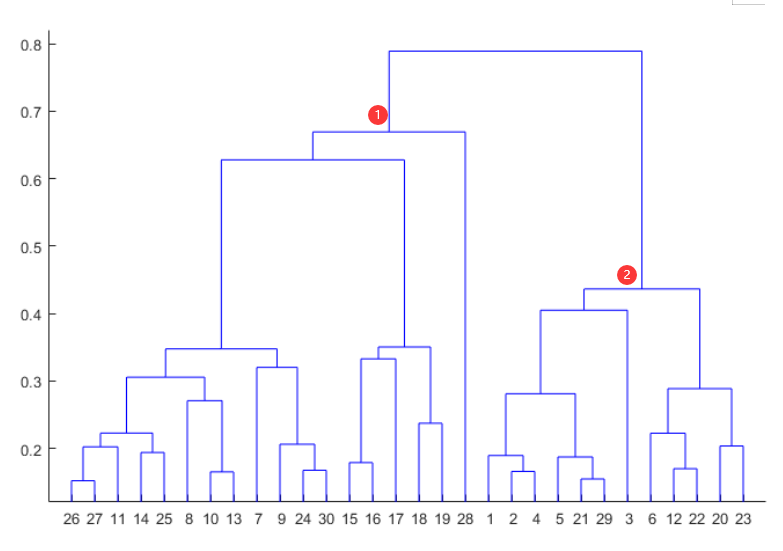
\includegraphics[width=12cm]{../../img/8.png}
	\caption{某一组层次聚类法结果} 
\end{figure}

如图所示的这一组中,我们总共选取了30个任务进行层次聚类,左边标记为1的18个任务进行一次打包,右边标记为2的12个任务进行一次打包。、
以此类推,我们将835个任务全部进行打包,打包结果如下:

\begin{table}[H]
	\centering
	\caption{打包结果}
\begin{tabular}{|c|c|c|c|}
	\hline
	打包任务数 & 个数 & 打包任务数 & 个数 \\ \hline
	20    & 2  & 10    & 7  \\ \hline
	19    & 1  & 9     & 4  \\ \hline
	18    & 2  & 8     & 6  \\ \hline
	17    & 1  & 7     & 2  \\ \hline
	16    & 3  & 6     & 8  \\ \hline
	15    & 3  & 5     & 4  \\ \hline
	14    & 2  & 4     & 9  \\ \hline
	13    & 4  & 3     & 11 \\ \hline
	12    & 5  & 2     & 14 \\ \hline
	11    & 3  &       &    \\ \hline
\end{tabular}
\end{table}
\vspace{-0.8cm}

将一个任务包里的多个任务看做一个整体,与其它未被打包的任务同为一个 任务,经过联合打包处理过后的任务数量由835个变为215个。

\subsubsection{打包任务的参数修正}

将任务打包之后,我们需要对任务包的参数进行重新修正。

\textbf{1.任务包的标价}
由于任务包是由多个任务组成,因此任务包的标价为所有任务标价之和。
k个任务组成的任务包标价如下:

\begin{equation}
{P_I} = \sum\limits_{i = 1}^k {{p_i}} 
\end{equation}

\textbf{2.任务包的位置坐标}

由于任务包是由几个距离邻近的任务组成的,因此,我们采用这几个位置坐标的平均坐标来作为位置包的坐标。

\begin{equation}
{X_I} = \frac{{\rm{1}}}{k}\sum\limits_{i = 1}^k {{x_i}} ,{Y_I} = \frac{{\rm{1}}}{k}\sum\limits_{i = 1}^k {{{\rm{y}}_i}} 
\end{equation}

\textbf{3.任务包的与用户之间的距离}

由于确定了任务包的位置坐标,任务包和用户之间的距离就可以用欧式距离来刻画。

\begin{equation}
{R_{{\rm{ij}}}} = \sqrt {{{\left( {{X_i}{\rm{ - }}{x_j}} \right)}^2} + {{\left( {{Y_i}{\rm{ - }}{y_j}} \right)}^2}} 
\end{equation}

之后将任务包等价普通的任务,重新构建多目标优化模型来求解任务定价和完成率。

目标函数:
\begin{equation}
\left\{ \begin{array}{l}
\min \sum\limits_{i = 1}^{215} {{p_i}} \\
\max \sum\limits_{i = 1}^{1864} {{C_i}} 
\end{array} \right.
\end{equation}

\begin{equation}
s.t.\left\{ \begin{array}{l}
{\rm{50}} \le {\rm{p}}{}_{\rm{i}} \le 100\\
{a_{ij}} = \frac{{G{n_j}{p_i}}}{{{r_{ij}}^2}}\\
{C_i} = \left\{ \begin{array}{l}
{\rm{1,}}{a_{ij}} \ge {a_i}\\
0,{a_{ij}} < {a_i}
\end{array} \right.\\
{{\rm{w}}_{{\rm{imax}}}} = {n_s} \times {m_i}\\
{n_s} = n - {n_d}\\
{{\rm{s}}_i} \in {n_s}\\
{{\rm{s}}_i} = \max ({a_{ij}}),{a_{ij}} > {a_i}\\
{s_i} = \max ({b_{s1}},{b_{s2}},...,{b_{sn}})
\end{array} \right.,i = 1,2,...,215,j = 1,2,...,1864
\end{equation}

  
求解之后,我们发现,在一共215个任务中,有185个任务被完成,完成率86.05\%,完成率较问题二的方案提升6.13\%。新方案总成本为45145元,较问题二降低8.7\%。说明新的定价方案优于问题二中的定价方案。


\subsection{问题四模型的建立及求解}
\subsubsection{数据可视化与任务打包}
\textbf{1.数据可视化}

附件三给了2066条新的任务经纬度数据,首先我们将其在地图上进行可视化,如下图所示。

\begin{figure}[H]
	\small
	\centering
	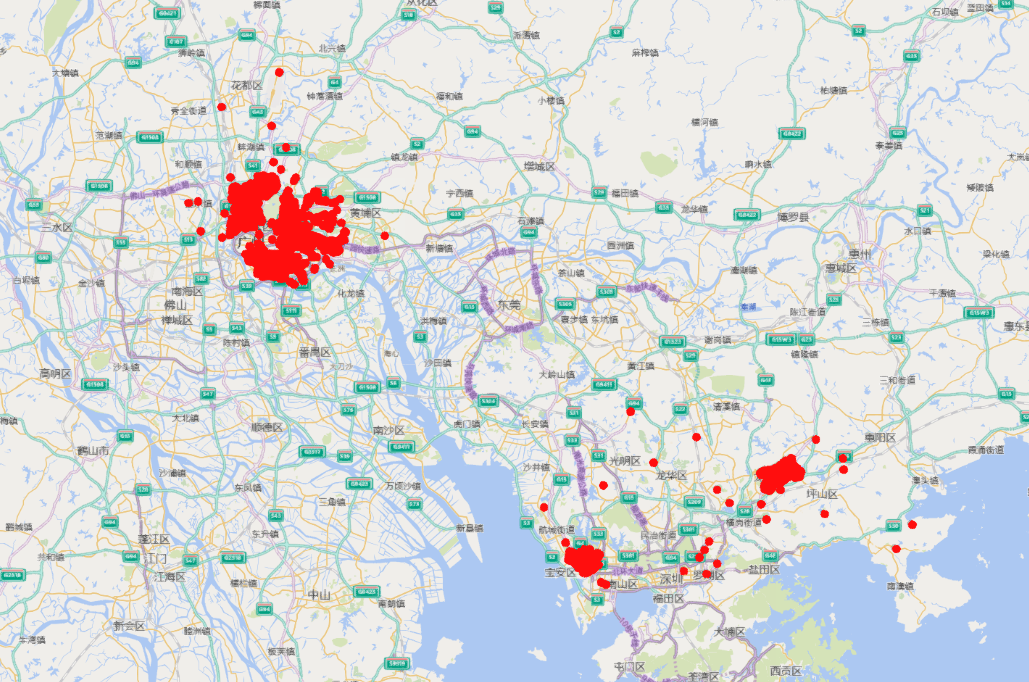
\includegraphics[width=12cm]{../../img/9.png}
	\caption{附件三任务分布图} 
\end{figure}

在图中我们发现,任务点主要集中在广州和深圳,和前面两问的情况相差不大,因此我们可以任务打包的基础上,调用神经网络模型来对新的任务进行定价和完成率的预测。

\textbf{2.任务的打包}

首先,我们通过数据预处理中的坐标转换法将这些任务的经纬度坐标转换成平面上的二维坐标。

之后,我们通过问题三中一样的层次聚类法,将2066个任务进行打包处理,处理结果如下表所示:

\begin{table}[H]
	\centering
	\caption{附件三任务打包表}
	\begin{tabular}{|c|c|c|c|}
		\hline
		打包任务数 & 个数 & 打包任务数 & 个数 \\ \hline
		20    & 8  & 10    & 8  \\ \hline
		19    & 13 & 9     & 6  \\ \hline
		18    & 15 & 8     & 2  \\ \hline
		17    & 11 & 7     & 16 \\ \hline
		16    & 5  & 6     & 12 \\ \hline
		15    & 8  & 5     & 11 \\ \hline
		14    & 7  & 4     & 14 \\ \hline
		13    & 6  & 3     & 15 \\ \hline
		12    & 4  & 2     & 14 \\ \hline
		11    & 5  &       &    \\ \hline
	\end{tabular}
\end{table}

经过打包处理过后的任务数量由835个变为385个。

\subsubsection{BP神经网络模型}
BP神经网络是是一种按误差逆传播算法训练的多层前馈网络,是目前应用最广泛的神经网络模型之一。

我们通过神经网络模型,来进行任务标价的确定和完成率的预测,输入变量为任务的经纬度数据,输出变量为任务的标价和完成情况。

\begin{figure}[H]
	\small
	\centering
	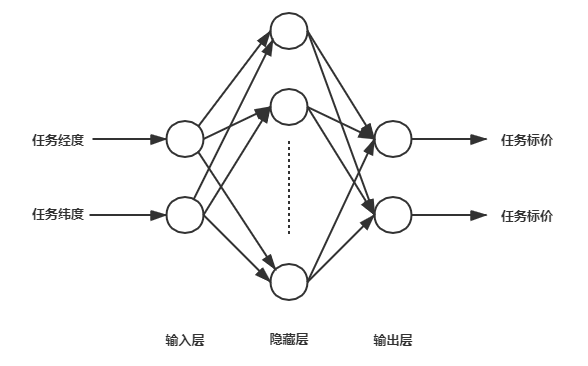
\includegraphics[width=12cm]{../../img/10.png}
	\caption{BP神经网络结构图} 
\end{figure}

代入第三问的数据进行训练,取70\%为数据集,15\%作为验证集,15\%作为测试集,训练结果如下图所示:

\begin{figure}[H]
	\small
	\centering
	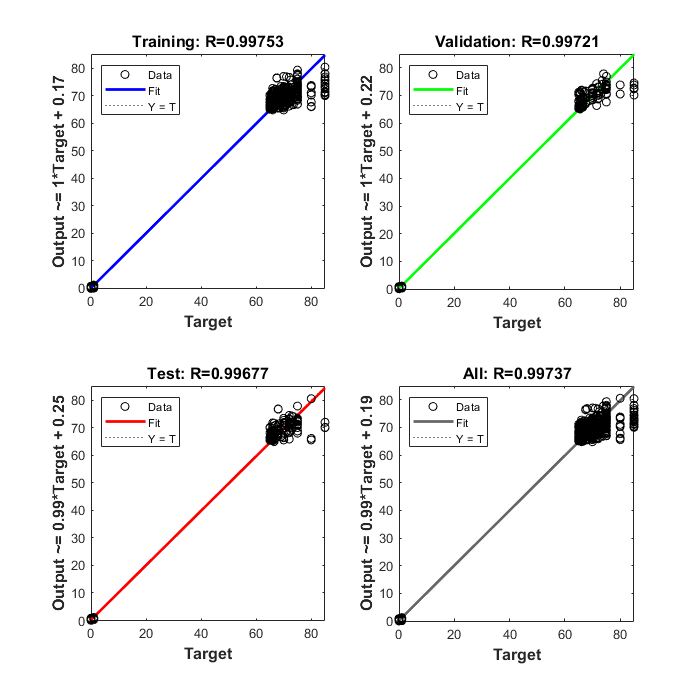
\includegraphics[width=12cm]{../../img/11.png}
	\caption{BP神经网络结果评测图} 
\end{figure}

图中可见总体的R值为0.997,接近1,拟合程度较好,说明该模型具有一定的准确性,我们可以利用它进行预测。

代入附件三的经纬度数据,我们得到了新的定价方案。

\begin{table}[H]
	\centering
	\caption{问题四任务标价与执行情况}
	\begin{threeparttable}       
		\begin{tabular}{|c|c|c|}
			\hline
			任务包编号    & 任务包标价    & 是否完成   \\ \hline
			1        & 65.5     & 1      \\ \hline
			2        & 138      & 1      \\ \hline
			3        & 322      & 0      \\ \hline
			4        & 64       & 1      \\ \hline
			5        & 58       & 1      \\ \hline
			\multicolumn{3}{|c|}{......} \\ \hline
			6        & 476      & 1      \\ \hline
			2        & 521      & 1      \\ \hline
			3        & 184      & 1      \\ \hline
			4        & 52       & 1      \\ \hline
			5        & 66       & 0      \\ \hline
		\end{tabular}
		\begin{tablenotes}
			\footnotesize
			\item 注:由于篇幅有限,这里仅展示部分数据。
		\end{tablenotes}
	\end{threeparttable}     
\end{table}


总共385个任务包,331包完成,任务完成率为85.97\%,价格成本为128436.28元。与前几问相比,任务完成率得到提高,平均单个任务价格为62.17元,成本也控制得较好。


\section{模型的评价}
\subsection{模型的优点}

1.进行了数据预处理,数据的准确率较高。

2.将经纬度转换为平面坐标进行计算,进一步提升了计算的准确性。

3.四个问题的模型联系紧密,层层递进。

\subsection{模型的缺点}

1.对任务和会员之间的距离仅考虑直线距离,未考虑其它因素造成距离上的改变。

2.吸引力阈值自主确定,具有一定的主观性。

3.BP神经网络模型可解释性较差。


\section{模型的推广}

本文模型的应用背景是基于智能手机和移动互联网的劳务众包平台\upcite{2018YOLOv3},在相似背景下的应用众多,如外卖应用,滴滴打车,快递跑腿服务平台等都涉及到商品定价与地理位置、会员积极程度的关系\upcite{2017YOLO9000}。


%参考文献
\bibliographystyle{unsrt}
\bibliography{reference}






\newpage
%附录
\begin{appendices}
\section{墨卡托投影法}
\begin{lstlisting}[language=matlab]
function [x,y]=ll_xy(lng, lat)
earthRad = 6378137.0;
x = ((lng .* pi) ./ 180) .* earthRad;
a = (lat .* pi) ./ 180;
y = (earthRad ./ 2) .* log((1.0 + sin(a)) ./ (1.0 - sin(a)));
end

tic
format long g
[x_p ,y_p] = ll_xy(x,y);
x_p = x_p - mean(x_p);
y_p = y_p - mean(y_p);
toc
 \end{lstlisting}
 
 \section{Kmeans-聚类算法}
\begin{lstlisting}[language=matlab]
opts = statset('Display','final');
%调用 Kmeans 函数
%X N*P 的数据矩阵
%Idx N*1 的向量,存储的是每个点的聚类标号
%Ctrs K*P 的矩阵,存储的是 K 个聚类质心位置
%SumD 1*K 的和向量,存储的是类间所有点与该类质心点距离之和
%D N*K 的矩阵,存储的是每个点与所有质心的距离;
[Idx,Ctrs,SumD,D] = kmeans(X,4,'Replicates',2,'Options',opts);
%画出聚类为 1 的点。X(Idx==1,1),为第一类的样本的第一个坐标;X(Idx==1,2为第二类的样本的第二个坐标
plot(X(Idx==1,1),X(Idx==1,2),'r.','MarkerSize',14)
hold on
plot(X(Idx==2,1),X(Idx==2,2),'b.','MarkerSize',14)
hold on
plot(X(Idx==3,1),X(Idx==3,2),'g.','MarkerSize',14)
hold on 
plot(X(Idx==4,1),X(Idx==4,2),'y.','MarkerSize',14)
%绘出聚类中心点,kx 表示是圆形
plot(Ctrs(:,1),Ctrs(:,2),'kx','MarkerSize',14,'LineWidth',4)
%legend('Cluster 1','Cluster 2','Cluster3','Centroids','Location','NW')
Ctrs
SumD
 \end{lstlisting}
 
 \section{层次聚类法}
 \begin{lstlisting}[language=python]
import pandas as pd
import seaborn as sns  # 用于绘制热图的工具包
from scipy.cluster import hierarchy  # 用于进行层次聚类,话层次聚类图的工具包
from scipy import cluster
import matplotlib.pyplot as plt
from sklearn import decomposition as skldec  # 用于主成分分析降维的包

from scipy.cluster.hierarchy import dendrogram, linkage, fcluster
from matplotlib import pyplot as plt

df = pd.read_excel("tempdata.xlsx", index_col=0, header=None)  #index_col=0指定数据中第一列是类别名称,PS:计算机程序一般从整数0开始计数,所以0就代表第一列
# df = df.T    #python默认每行是一个样本,如果数据每列是一个样本的话,转置一下即可

X = df.index
# print (X)
# method是指计算类间距离的方法,比较常用的有3种:
# single:最近邻,把类与类间距离最近的作为类间距
# average:平均距离,类与类间所有pairs距离的平均
# complete:最远邻,把类与类间距离最远的作为类间距
Z = linkage(X, 'average')
f = fcluster(Z, 4, 'distance')
fig = plt.figure()
dn = dendrogram(Z)
plt.show()

 \end{lstlisting}
\end{appendices}

\end{document} 